\documentclass[11pt]{amsart}

\usepackage[english]{babel}
\usepackage {amsmath} 
\usepackage{amssymb}
\usepackage{amsfonts}
\usepackage{amsthm}
\usepackage{graphicx}
\usepackage[dvipsnames]{xcolor}
\usepackage{lipsum}
\usepackage[colorlinks,linkcolor=blue, citecolor=blue,urlcolor=blue]{hyperref}
\usepackage[backend=bibtex]{biblatex}
\usepackage[colorinlistoftodos]{todonotes}

\newcommand{\info}[1]{\todo[linecolor=OliveGreen,backgroundcolor=OliveGreen!25,bordercolor=OliveGreen]{#1}}
\newcommand{\unsure}[1]{\todo[linecolor=red,backgroundcolor=red!25,bordercolor=red]{#1}}
\newcommand{\change}[1]{\todo[linecolor=Plum,backgroundcolor=Plum!25,bordercolor=Plum]{#1}}

%% Environments for theorems, etc.. 
\theoremstyle{theorem} % set the style for the following theorems
\newtheorem{thm}{Theorem}[section] %\newtheorem{name}{display-text}[numbered-within]
\newtheorem{lem}[thm]{Lemma} %\newtheorem{name}[numbered-like]{display-text}
\newtheorem{cor}[thm]{Corollary}
\newtheorem{prop}[thm]{Proposition}
\newtheorem{alg}[thm]{Algorithm}
\theoremstyle{definition}       
\newtheorem{defn}[thm]{Definition}
\newtheorem{conj}[thm]{Conjecture}
\theoremstyle{example}                     
\newtheorem{prob}[thm]{Problem}
\theoremstyle{remark}                       
\newtheorem{exmp}[thm]{Example}
\newtheorem{rem}[thm]{Remark}
\newtheorem{claim}[thm]{Claim}  
\renewcommand{\theclaim}{}

\numberwithin{equation}{section}

\newcommand{\R}{\mathbb{R}}
\newcommand{\Q}{\mathbb{Q}}
\newcommand{\N}{\mathbb{N}}
\newcommand{\Z}{\mathbb{Z}}
\DeclareMathOperator{\rank}{rank}
\DeclareMathOperator{\dimension}{dim}
\DeclareMathOperator*{\supp}{supp}
\DeclareMathOperator{\spn}{span}


\addbibresource{wavelet.bib}


\author{Jason Ngo}
\begin{document}
	\begin{lem}[Average of continuous function over dyadic intervals, {\cite[295]{pinsky}}] \label{lem:average} \quad
		\begin{enumerate}
			\item If $ g \in C_0(\R) $, we have $ \| P_{-m}g \|_\infty \to 0 $ when $ m \to \infty $.
			\item If $ f \in L^2(\R) $, we have $ \| P_{-m}f \|_2 \to 0 $ when $ m \to \infty $.
		\end{enumerate}
	
		\begin{proof}
			We will first prove (1).
		\end{proof}
	\end{lem}
	
	\begin{exmp}
		Consider $ f(x) = e^{-x} \sin 2\pi x $ for $ x \in (0,1) $.
		
		See Figure \ref{fig:approximations} 
	\end{exmp}
	
	
	
	\begin{figure}
		\centering
		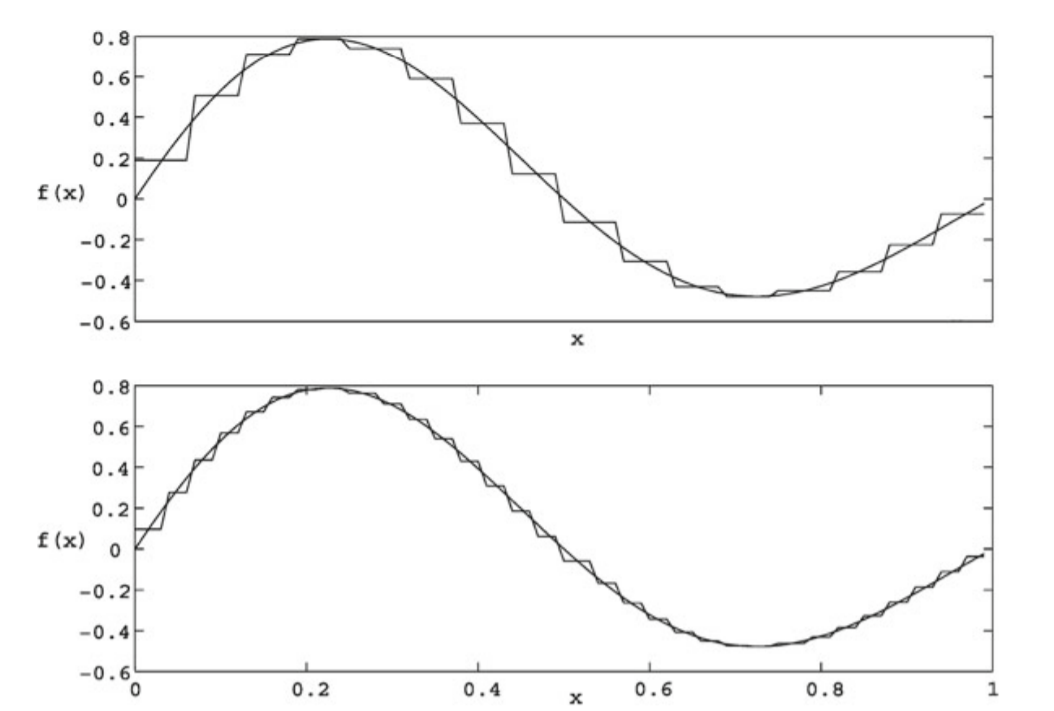
\includegraphics[width=0.7\linewidth]{img/approximations}
		\caption{Approximations of $ f(x) = e^{-x} \sin{2\pi x} $ using Haar wavelets \cite{lepik}}
		\label{fig:approximations}
	\end{figure}
	
	
	-------------------------
	
	Let $ C_c (\R) $ denote the set of continuous functions such that $ \supp(f) $ is a compact set.
	Since we know that $ C_c(\R) $ is dense in $ L^2(\R) $\footnote{The proof for this claim can be found in \cite[326]{farrell}.}, it suffices to show $ C_c (\R) $ is spanned by the Haar system.\info{more explanation needed, maybe a small $ \epsilon $ proof.} \change{paraphrase from \cite{davidson}}Each such function with compact support is te finite sum of (piecewise) continuous functions supported on an interval $ [m, m+1) $. But our basis is invariant under integer translations, so it is enough to show that a function on $ [0,1) $ is spanned by the Haar system.
	
	\vspace{12pt}
	In the next section, we will prove that the Haar system spans $ L^2(0,1) $. To do this, consider the functions $ \{ \varPsi_{j,k} \} $ in the Haar system that are supported on $ [0,1) $, namely $ 0 \leq k \leq 2^j $ for each $ j \geq 0 $. We define the inner product expansion as follows:
	
	\begin{defn}[Inner Product Expansion, {\cite[409]{davidson}}] \label{def:expansion}
		Set $ \varphi = \chi_{[0,1)} $. Define the sequence of partial sums $ H_nf $ to be:
		\[ H_n f(x) = \langle f, \varphi \rangle \varphi(x) + \sum_{j=0}^{n-1} \sum_{k=0}^{2^j-1} \langle f, \varPsi_{j,k} \rangle \varPsi_{j,k} (x). \]
	\end{defn}
	
	\unsure{explanation needed.}The first term $ \langle f, \varphi \rangle $ is to consider $ f $ on $ [0,1) $ only.
	The \emph{Haar coefficients} are the inner products $ \langle f, \varPsi_{j,k} \rangle $ in the expansion.                                         
	\info{some description of $ H_nf $}
	
	\change{make the sure notations are consistent among $ j,k,n $}
	
	\begin{lem}[{\cite[410]{davidson}}]
		Let $ f \in L^2 (0,1) $. Then $ H_n f $ is the unique function that is constant on each dyadic interval of length $ 2^{-n} $ in $ [0,1] $ and satisfies
		\[ H_nf(x) = 2^n \int_{} \]
	\end{lem}
	
	\begin{lem}
		Let $ f \in L^2(0,1) $. Then $ H_nf $ converges to $ f $ in the $ L^2 $ norm. Consequently, the Haar system is an orthonormal basis for $ L^2(0,1) $. Moreover, if $ f $ is continuous on $ [0,1] $, then $ H_nf $ converges uniformly to $ f $.
	\end{lem}
	
	\section{whatever}
	\begin{thm} \label{convergence}
		If $ f \in C_0(\R) $, then the series $ \sum_{j,k \in \Z} \langle f, \varPsi_{j,k} \rangle \varPsi_{j,k} $ converges to $ f $ uniformly on $ \R $.
	\end{thm}
	
	\section{Approximations using Haar wavelets}
	
	
-----------------------------------

\begin{rem}
	$ \varPsi_{j,k} $ has width of $ 2^{-j} $ and is centered about $ k 2^{-j} $. Furthermore, we can see that:
	\begin{enumerate}
		\item $ \int_{\R} \varPsi(x)dx = 0 $, which makes $ \varPsi $ a wave.
		\item  $ \int_{\R} \varPsi(x)^2dx = 1 $, i.e. the norm of $ \varPsi $ is 1.
	\end{enumerate}
\end{rem}	

\begin{quote}
	The child wavelets $ \varPsi_{j,k} $ are simply dilated and translated versions of the mother wavelet multiplied with the normalization factor 2j/2. The normalization factor is there so that the dilated and translated Haar function satisfies property (2) in the wavelet	definition.
\end{quote}

Observe that all $ \varPsi_{j,k} $ are generated by shifting and scaling\footnote{The dilations here are taken to be powers of 2.} the wavelet $ \varPsi $ and that each $ \varPsi_{j,k} $ is normalized so that $ \| \varPsi_{j,k}\|_2 = \|\varPsi\|_2 = 1 $ for all $ j,k \in \Z $.

---

i.e., the intervals on which they are non-zero are different; therefore, when the two functions multiply together, the result must be zero (therefore the 2-norm is 0). Thus, they are orthogonal. 
\begin{quote}
	Now, if $ j < j' $, then $ \varphi $ and $ \varPsi_{j,k} $ are constant on the support of $ \varPsi_{j',k'} $. Since $ \int_0^1 \varPsi_{j,k}(x) = 0 $ for all $ j $ and $ k $, it now follos that these functions are pairwise orthogonal.
\end{quote}

\section{Useful quotes}
\begin{quote}
	Wavelets are local functions that enable us to cut up data into different layers of frequency. A wavelet basis is formed by translating and dilating a small wave, making it
	possible to analyze data at different scales. Although wavelet analysis is promising, it
	has not entered mainstream study of economic phenomena. The aim of this thesis is to
	give an intuitive theoretical understanding of wavelets, and describe how they can be
	used in time series analysis. Applications for economic time series are presented, as well
	as some thoughts of how the field of economics will progress due to wavelet analysis.
\end{quote}


\section{Annotated Bibliography}
\begin{enumerate}
	\item \fullcite{davidson_real_2002}
	
	\smallskip
	This textbook is my primary source for proofs of orthonormal basis. Though terse, the book introduces the lemmas and proofs in a logical way, starting with proving the Haar system is orthonormal and then expand it to the basis for $L^2(\R)$.
	
	\item \fullcite{Frazier_1999}
	
	\smallskip
	This textbook is very introductory, including a lot of examples and step-by-step proof for the properties of wavelets. Furthermore, it also has a nice description of the FBI Fingerprint Compression application using Haar Wavelets Analysis.	
	
	\item \fullcite{Gomes_Velho_2015}
	
	\smallskip
	Although this textbook is not very proof-heavy, it brings up a lot of cool wavelet examples that pertain to image compression, one of which being the Blur Derivative that I can talk about in my first draft.
\end{enumerate}	
	
\end{document}